% Source: moreBoseEinstein.pdf, pages 1-9. Title on the source: "Further applications of Bose-Einstein
% statistics". No lecture number.
\subsection{Blackbody radiation}

For photons in thermal equilibrium at temperature $T$,
\begin{equation}
  \ev{n_r} = \frac{1}{e^{\beta E_r}-1}
\end{equation}
is the number of photons with energy $E_r$ in a state $r$. Recall that since photons are self-conjugate, $\mu = 0$.

As a function of wavevector $\mathbf k$, the number of photon states with wavevector between $\mathbf k$ and
$\mathbf k+\dd\mathbf k$ is
\begin{equation}
  \dd N = \frac{L^3\dd^3k}{(2\pi)^3} = \frac{V\dd^3k}{(2\pi)^3}.
\end{equation}
Now the frequency is $\nu = c/\lambda$, so $\omega = 2\pi\nu = 2\pi c/\lambda = ck$, where $c$ is the velocity of
light, $\lambda$ is the wavelength, and $k = 2\pi/\lambda$; $k = |\mathbf k|$. From the Maxwell equations in vacuum,
$\boldsymbol\nabla\times\mathbf E = -(1/c)\partial\mathbf B/\partial t$,
$\boldsymbol\nabla\times\mathbf B = (1/c)\partial\mathbf E/\partial t$, $\boldsymbol\nabla\cdot\mathbf E = 0$ and
$\boldsymbol\nabla\cdot\mathbf B = 0$ $\Rightarrow$ the electromagnetic wave equations
\begin{equation}
  \left(\nabla^2-\frac{1}{c^2}\frac{\partial^2}{\partial t^2}\right)\mathbf E = 0,\qquad
  \left(\nabla^2-\frac{1}{c^2}\frac{\partial^2}{\partial t^2}\right)\mathbf B = 0,
\end{equation}
with $\mathbf E\perp\hat{\mathbf k}$, $\mathbf B\perp\hat{\mathbf k}$, $\mathbf E\perp\mathbf B$. The electromagnetic waves have 2
polarizations. Denote $f(k)$ as the differential number of photon states per unit volume with wave vector between $\mathbf k$ and
$\mathbf k+\dd\mathbf k$:
\begin{equation}
  f(k)\dd k = 2\left(\frac{1}{e^{\beta E_k}-1}\right)\cdot\frac{\dd^3k}{(2\pi)^3};
\end{equation}
$\dd^3k = k^2\dd k\,\dd\Omega_k = 4\pi k^2\dd k$, and the photon energy is $E_k = h\nu = \hbar\omega$, where $h$ is Planck's
constant and $\omega = ck$, so we can write this as
\begin{equation}
  f(\omega)\dd\omega = \frac{2(4\pi)}{(2\pi c)^3}\left(\frac{1}{e^{\beta\hbar\omega}-1}\right)\omega^2\dd\omega
  = \frac{1}{\pi^2c^3}\frac{\omega^2\dd\omega}{(e^{\beta\hbar\omega}-1)}.
\end{equation}
Then the average energy density in the EM radiation per unit volume, for photons with angular frequencies $\omega$ to
$\omega+\dd\omega$, is
\begin{equation}
  \boxed{U(\omega)\dd\omega = \frac{\hbar}{\pi^2c^3}\frac{\omega^3\dd\omega}{(e^{\beta\hbar\omega}-1)}}.
\end{equation}
Now define a dimensionless variable $y = \beta\hbar\omega = \hbar\omega/(\kB T)$, so $\omega = (\kB T/\hbar)y$:
\begin{equation}
  \Rightarrow\quad U(\omega)\dd\omega = \frac{\hbar}{\pi^2c^3}\left(\frac{\kB T}{\hbar}\right)^4\frac{y^3\dd y}{(e^y-1)}
  = \boxed{\frac{1}{\pi^2}\frac{(\kB T)^4}{(\hbar c)^3}\frac{y^3\dd y}{(e^y-1)}}
\end{equation}
(M.~Planck (1900); Nobel Prize 1918).

\begin{diagram}
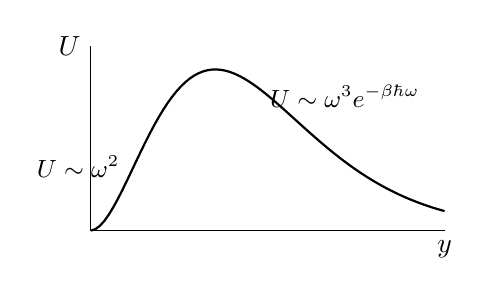
\begin{tikzpicture}[scale=0.9]
  \draw (0,0) -- (5,0) node[below] {$y$}; \draw (0,0) -- (0,2.6) node[left] {$U$};
  \draw[thick,domain=0.01:5,samples=80] plot (\x,{1.6*(\x*1.6)^3/(exp(\x*1.6)-1)});
  \node[font=\small,anchor=east] at (0.55,0.9) {$U\sim\omega^2$};
  \node[font=\small,anchor=west] at (2.4,1.9) {$U\sim\omega^3e^{-\beta\hbar\omega}$};
\end{tikzpicture}
\diagramcaption{The Planck distribution.}
\end{diagram}

For $y\ll 1$, i.e.\ $\hbar\omega\ll\kB T$, expand the denominator:
$y^3\dd y/((1+y+\ldots)-1) = y^2\dd y = (\beta\hbar)^3\omega^2\dd\omega$, and
\begin{equation}
  U(\omega)\dd\omega = \frac{1}{\pi^2}\frac{(\kB T)^4}{(\hbar c)^3}\left(\frac{\hbar}{\kB T}\right)^3\omega^2\dd\omega
  = \frac{\kB T}{\pi^2c^3}\omega^2\dd\omega,
\end{equation}
the classical Rayleigh--Jeans law (note how $\hbar$ cancels out). So we recover the classical Rayleigh--Jeans result at low
frequencies. The recognition that this classical relation gave an ``ultraviolet catastrophe'', namely $U(\omega)\to\infty$ as
$\omega\to\infty$, was a key motivation for the idea that electromagnetic radiation is composed of particles, photons, with
energy $E = \hbar\omega$. Einstein used this to explain the photoelectric effect (1905), for which he got the 1921 Nobel Prize.
For $\hbar\omega\gg\kB T$, i.e.\ $y\gg 1$, where $y = \beta\hbar\omega$,
\begin{equation}
  U(\omega)\dd\omega\simeq\frac{1}{\pi^2}\frac{1}{\beta^4(\hbar c)^3}\underbrace{\frac{y^3\dd y}{e^y-1}}_{y^3e^{-y}\dd y = \beta^4\hbar^4\omega^3e^{-\beta\hbar\omega}\dd\omega}
  = \frac{\hbar}{\pi^2}\left(\frac{\omega}{c}\right)^3e^{-\beta\hbar\omega}\dd\omega,
\end{equation}
which decreases (exponentially rapidly) to 0 as $\hbar\omega/(\kB T)\to\infty$.

The total energy per volume in the thermal photons (``blackbody radiation'') is
\begin{equation}
  U = U(T) = \int_0^\infty U(T,\omega)\dd\omega = \frac{1}{\pi^2}\frac{(\kB T)^4}{(\hbar c)^3}\underbrace{\int_0^\infty\frac{y^3\dd y}{(e^y-1)}}_{=\pi^4/15},
  \qquad\boxed{U(T) = \frac{\pi^2}{15}\frac{(\kB T)^4}{(\hbar c)^3}}.
\end{equation}

\subsubsection*{Radiated power and Wien's law}

A related quantity is the power per unit area emitted by a thermal bath of photons, at angular frequencies between $\omega$ and
$\omega+\dd\omega$. Recall the Poynting vector $\mathbf S\propto c(\mathbf E\times\mathbf B)\propto c(\mathbf E^2+\mathbf B^2)\propto cU$
($\mathbf E$ and $\mathbf B$ have the same dimensions in Gaussian units)
\begin{equation}
  \Rightarrow\quad P(\omega)\dd\omega = \frac{c}{4}U\dd\omega = \frac{\hbar}{4\pi^2c^2}\frac{\omega^3\dd\omega}{(e^{\beta\hbar\omega}-1)}
  = \frac{(\kB T)^4}{4\pi^2\hbar^3c^2}\frac{y^3\dd y}{(e^y-1)},\qquad y = \beta\hbar\omega,
\end{equation}
\begin{equation}
  P_{\text{tot}} = \int_0^\infty P(\omega)\dd\omega = \frac{(\kB T)^4}{4\pi^2\hbar^3c^2}\underbrace{\int_0^\infty\frac{y^3\dd y}{e^y-1}}_{\pi^4/15}
  = \left(\frac{\pi^2\kB^4}{60\hbar^3c^2}\right)T^4 = \sigma T^4,
\end{equation}
where $\sigma = \pi^2\kB^4/(60\hbar^3c^2) = 5.67\times 10^{-8}\ \text{Watts}/(\text{m}^2\text{K}^4)$ is the
Stefan--Boltzmann constant. Since $\nu = c/\lambda$, $\dd\nu = -(c/\lambda^2)\dd\lambda$; reexpress this as a function of
$\lambda$:
\begin{equation}
  \Rightarrow\quad P(\lambda)\dd\lambda\propto\lambda^{-3}\left(\frac{\dd\lambda}{\lambda^2}\right)\Big/\left[\exp\left(\frac{hc}{\lambda\kB T}\right)-1\right],
\end{equation}
with a maximum at
\begin{equation}
  \boxed{\lambda_{\max} = \frac{2.90\times 10^{-3}\ \text{m}\cdot\text{K}}{T}}\qquad\text{(Wien Displacement Law)}.
\end{equation}

\begin{diagram}
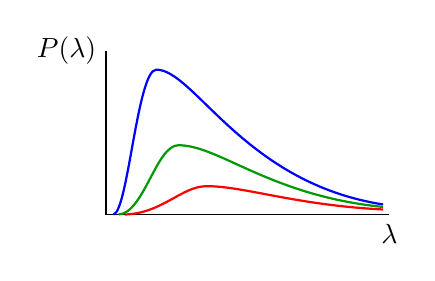
\begin{tikzpicture}[scale=0.8]
  \draw (0,0) -- (4.5,0) node[below] {$\lambda$}; \draw (0,0) -- (0,2.6) node[left] {$P(\lambda)$};
  \draw[thick,red] (0.3,0) .. controls (0.9,0.02) and (1.2,0.45) .. (1.6,0.45) .. controls (2.2,0.45) and (3,0.15) .. (4.4,0.08);
  \draw[thick,green!60!black] (0.2,0) .. controls (0.6,0.02) and (0.8,1.1) .. (1.15,1.1) .. controls (1.8,1.1) and (2.6,0.3) .. (4.4,0.12);
  \draw[thick,blue] (0.12,0) .. controls (0.35,0.05) and (0.5,2.3) .. (0.8,2.3) .. controls (1.4,2.3) and (2.2,0.5) .. (4.4,0.16);
\end{tikzpicture}
\diagramcaption{As $T$ increases, the $\lambda$ at the maximum decreases and the overall power emitted increases.}
\end{diagram}

The chromosphere (outer layer) of a G-type star (the sun is spectral type G2) has a temperature $T\sim 5\times 10^3$~K
$\Rightarrow\lambda_{\max} = 2.90\times 10^{-3}\ \text{m}\cdot\text{K}/(5\times 10^3\ \text{K})\sim 0.6\times 10^{-6}\ \text{m} = 600\ \text{nm} = 6000$~\AA.
Because the power peaks at this $\lambda$, the color of the sun is creamy yellow. Cooler stars appear redder, since a lower $T$ of the
chromosphere $\Rightarrow$ larger $\lambda_{\max}$, e.g.\ Aldebaran (type K5), Betelgeuse (M2); Sirius (A0) is blue-white, Rigel (B8)
white. The stellar spectral series is O B A F G K M, from high $T$ to low $T$.

Closer to hand, one can observe this $T$ dependence of $P(\lambda)$ with hot metal. As $T$ increases through $\sim 10^3$~K, iron
appears reddish, then orange; at these temperatures, one can hammer and shape iron or steel. The melting temperature of Fe is
$T_m = 1.81\times 10^3$~K; viewing liquid iron or steel being poured in a steel factory, it appears $\sim$ white.

\subsubsection*{The cosmic microwave background}

An important application of these results for thermal EM radiation has been in cosmology, specifically the observation and study of
the cosmic microwave background radiation, CMB. After the Big Bang, when the temperature $T$ was larger than $\sim$ eV, atoms and
molecules could not exist; any incipient Coulombic bound state would be ionized by the photons, so (for $T<\Lambda_{QCD}$) there was a
plasma of protons and electrons (and $\alpha$ particles after primordial nucleosynthesis). Thus photons did not propagate freely but
scattered from the e's and p's and $\alpha$'s. As $\kB T$ decreased below $\sim 1$~eV, the e's formed atoms: $(ep)$, hydrogen, and
$ee\alpha$ = He, helium (with H $\sim 75\%$ and He $\sim 25\%$ of usual matter). After this time, the photons could propagate
essentially freely (except for absorption by dust from later matter aggregation). As the universe cooled, the photon energies were
red-shifted; this shifted the energies down by a factor of $\sim 10^3$, to $T\sim 2.73$~K:
\begin{equation}
  \lambda_{\max} = \frac{2.90\times 10^{-3}\ \text{m}\cdot\text{K}}{2.73\ \text{K}}\sim 1\ \text{mm}.
\end{equation}
This corresponds to a microwave frequency, $\nu = c/\lambda = 3.0\times 10^8\ \text{m/s}/(10^{-3}\ \text{m})\sim 3\times 10^{11}\ \text{Hz}\sim 300$~GHz.

The CMB was first observed by A.~Penzias and R.~Wilson at Bell Labs Holmdel (NJ) in 1965 using microwave antennas (Nobel Prize, 1978).
Later, measurements were made using ground-based and space missions that confirmed that the observed $P(\omega)$ does agree with the
blackbody formula: COBE (Cosmic Background Explorer, 1989--93; Nobel Prize 2006 to J.~Mather and G.~Smoot); WMAP (Wilkinson
Microwave Anisotropy Probe, 2001--2010); Planck (2009--2013). $T_{\text{CMB}} = 2.7255\pm 0.0003$~K is very precisely measured, and
the small ($\sim 10^{-5}$) fluctuations measured by WMAP and Planck have given important information about these seeds for LSS =
large-scale structure formation.

We next proceed to discuss another application of Bose--Einstein statistics, to quantized lattice vibrations: phonons.

\subsection{Phonons and conduction electrons}
\subsubsection*{Lattice vibrations, phonons and specific heat capacities}

Consider a solid consisting of $N$ particles, atoms (e.g.\ Fe, Cu, \ldots) or molecules (ice, \ldots). These have equilibrium positions
$\mathbf r_i^{(0)}$ at lattice sites, but vibrate about these positions, so their actual positions are at $\mathbf r_i$,
$i = 1,\ldots,N$. Denote the deviations from the equilibrium positions as $\boldsymbol\xi_i = \mathbf r_i-\mathbf r_i^{(0)}$. The
velocity of the $i$th atom or molecule is $\mathbf v_i = \dd\boldsymbol\xi_i/\dd t$. The real application is to dimension $d = 3$, but
let us keep $d$ general. The kinetic energy is
\begin{equation}
  E_{\text{kin}} = \sum_{i=1}^N\frac{m\mathbf v_i^2}{2} = \frac{m}{2}\sum_{i=1}^N\sum_{\alpha=1}^dv_{i\alpha}^2 .
\end{equation}
The potential energy is
\begin{equation}
  V(\mathbf r_1,\ldots,\mathbf r_N) = \underbrace{V(\mathbf r_1^{(0)},\ldots,\mathbf r_N^{(0)})}_{V_0}
  + \sum_{i=1}^N\sum_{\alpha=1}^d\left(\frac{\partial V}{\partial r_{i\alpha}}\right)_0\xi_{i\alpha}
  + \frac{1}{2!}\sum_{i,j=1}^N\sum_{\alpha,\beta=1}^d\left(\frac{\partial^2V}{\partial r_{i\alpha}\partial r_{j\beta}}\right)_0\xi_{i\alpha}\xi_{j\beta}
\end{equation}
to quadratic order in small deviations, where $(\ )_0$ means evaluation at the equilibrium positions, and
$\partial V/\partial r_{i\alpha} = \partial V/\partial\xi_{i\alpha}$.

The constant term $V_0$ is arbitrary and will not affect the dynamics. The linear term involves
$\partial V/\partial r_{i\alpha} = -F_{i\alpha}$, the force on the $i$th particle in direction $\alpha$ at
$r_{i\alpha}^{(0)}$; this $=0$ by the definition of the equilibrium points $\mathbf r_i^{(0)}$. Equivalently, it is the slope of $V$
as a function of $r_{i\alpha}$ and must be zero at the minimum. The summand of the quadratic term is symmetric in $(i,j)$ and
$(\alpha,\beta)$, so we can define
\begin{equation}
  A_{i\alpha,j\beta}\equiv\left(\frac{\partial^2V}{\partial r_{i\alpha}\partial r_{j\beta}}\right)_0
\end{equation}
and diagonalize $A$, obtaining the normal modes of this system.

This system thus has the form of a simple harmonic oscillator (SHO). Recall the Hamiltonian for a SHO:
\begin{equation}
  \Ham_{\text{SHO}} = \frac{1}{2}m\dot{\mathbf r}^2 + \frac{\kappa}{2}(\mathbf r-\mathbf r^{(0)})^2,
\end{equation}
where $\kappa$ is the ``spring constant''. Defining rescaled coordinates $\mathbf q = \sqrt m(\mathbf r-\mathbf r^{(0)})$,
$\Ham_{\text{SHO}} = (1/2)\dot{\mathbf q}^2 + (1/2)\omega^2\mathbf q^2$, where $\omega = \sqrt{\kappa/m}$ is the oscillation (angular)
frequency. Here we have a Hamiltonian describing the quantized vibrations of the atoms or molecules about their equilibrium positions in
the form of a SHO with $d\cdot N$ coordinates. The solution for the quantum mechanical energy eigenvalues is
$E_j = \hbar\omega_j(1/2+n_j)$ for each oscillator $j = 1,\ldots,d\cdot N$. The total wavefunction is $\prod_j|n_j\rangle$. So
\begin{equation}
  E_{\text{tot}} = V_0 + \sum_{j=1}^{d\cdot N}\left(\frac{1}{2}+n_j\right)\hbar\omega_j = \tilde V_0 + \sum_{j=1}^{d\cdot N}n_j\hbar\omega_j .
\end{equation}
Then the partition function is
\begin{align}
  Z &= \sum_{\{n_j\}}e^{-\beta E} = \sum_{\{n_j\}}e^{-\beta\sum_jn_j\hbar\omega_j}
     = \sum_{\{n_j\}}\left[\prod_{j=1}^{d\cdot N}e^{-\beta n_j\hbar\omega_j}\right]
     = \prod_{j=1}^{d\cdot N}\frac{1}{(1-e^{-\beta\hbar\omega_j})},
\end{align}
using, for each, $\sum_{n_1=0}^\infty e^{-\beta n_1\hbar\omega_1} = \sum_{n_1=0}^\infty x^{n_1} = 1/(1-x)$ with
$x = e^{-\beta\hbar\omega_1}$; $\ln Z = -\sum_{j=1}^{d\cdot N}\ln(1-e^{-\beta\hbar\omega_j})$,
\begin{equation}
  U = -\pder{}{\beta}\ln Z = +\pder{}{\beta}\sum_{j=1}^{d\cdot N}\ln\left(1-e^{-\beta\hbar\omega_j}\right)
    = \sum_{j=1}^{d\cdot N}\frac{\hbar\omega_je^{-\beta\hbar\omega_j}}{(1-e^{-\beta\hbar\omega_j})},
\end{equation}
i.e.
\begin{equation}
  U = \sum_{j=1}^{d\cdot N}\frac{\hbar\omega_j}{(e^{\beta\hbar\omega_j}-1)}.
\end{equation}
So one sees that the quantized lattice vibrations behave as bosons; they are called phonons because excitations propagate at the speed
of sound. The associated energy has the form $U = \sum_jE_jn_j$, where $n_j = 1/(e^{\beta\hbar\omega_j}-1)$ is the
Bose--Einstein occupation number.

In a real solid, the normal-mode frequencies are very closely spaced, so one replaces the sum by an integral, with a density-of-states
function $\mathcal D(\omega) = \dd N_{\text{osc}}/\dd\omega$, where $N_{\text{osc}}$ = \# oscillator states:
\begin{equation}
  \ln Z = -\int_0^\infty\dd\omega\,\mathcal D(\omega)\ln(1-e^{-\beta\hbar\omega}),\qquad
  U = \int_0^\infty\dd\omega\,\mathcal D(\omega)\frac{\hbar\omega}{(e^{\beta\hbar\omega}-1)}.
\end{equation}
The specific heat capacity is $C_v = \left(\dd U/\dd T\right)_V = -\kB\beta^2\dd U/\dd\beta$, and
$(\dd/\dd\beta)(e^{\beta\hbar\omega}-1)^{-1} = -(e^{\beta\hbar\omega}-1)^{-2}\hbar\omega e^{\beta\hbar\omega}$ (N.B.:
$C_v\simeq C_p$ for a solid), so
\begin{equation}
  C_v = \kB\beta^2\int_0^\infty\dd\omega\,\mathcal D(\omega)\frac{(\hbar\omega)^2e^{\beta\hbar\omega}}{(e^{\beta\hbar\omega}-1)^2},
  \quad\text{i.e.}\quad
  \boxed{C_v = \kB\int_0^\infty\dd\omega\,\mathcal D(\omega)\frac{(\beta\hbar\omega)^2e^{\beta\hbar\omega}}{(e^{\beta\hbar\omega}-1)^2}}.
\end{equation}
This is a general result. In an actual solid, $\mathcal D(\omega)$ is a complicated function of $\omega$.

\paragraph{The Debye model.}

P.~Debye developed a simple approximate model for $\mathcal D(\omega)$, according to which the phonon oscillation frequencies extend up
to a finite value, $\omega_D$, the Debye frequency. This is reasonable since at sufficiently high $\omega$, the substance would melt.
From $\lambda$ = (velocity of sound) $\times$ (period of oscillation) $= v_s/\nu$, i.e.\
$\lambda\!\!\!^- = 1/k = v_s/\omega$, we have $\omega = v_sk$. The number of oscillation modes up to $k$ is (oscillations can
occur in any of $d$ directions)
\begin{equation}
  d\cdot L^d\int\frac{\dd^dk}{(2\pi)^d} = \frac{d\cdot V}{(2\pi)^d}\int_0k^{d-1}\dd k\underbrace{\int\dd\Omega}_{A_d}
  = \frac{d\cdot V}{(2\pi)^d}\cdot\frac{k^d}{d}\cdot A_d = \frac{V\omega^dA_d}{(2\pi v_s)^d},
\end{equation}
where $A_d = 2\pi^{d/2}/(\Gamma(d/2))$, e.g.\ $A_3 = 2\pi^{3/2}/(\Gamma(3/2)) = 4\pi$ (with $\Gamma(1/2) = \sqrt\pi$,
$\Gamma(3/2) = (1/2)\Gamma(1/2) = \sqrt\pi/2$). So
\begin{equation}
  \mathcal D(\omega) = \frac{\dd N_{\text{osc}}}{\dd\omega} = \frac{d\cdot V\cdot\omega^{d-1}A_d}{(2\pi v_s)^d};
\end{equation}
now $N_{\text{osc}} = d\cdot N = \int_0^\infty\dd\omega\,\mathcal D(\omega)$, and in the Debye model, since $\omega\le\omega_D$,
\begin{equation}
  \Rightarrow\ d\cdot N = \int_0^{\omega_D}\dd\omega\,\mathcal D(\omega) = \frac{d\cdot V\cdot A_d}{(2\pi v_s)^d}\underbrace{\int_0^{\omega_D}\dd\omega\,\omega^{d-1}}_{\omega_D^d/d}
  = \frac{V\cdot A_d\omega_D^d}{(2\pi v_s)^d},
\end{equation}
so $d\cdot\left(N/V\right)\cdot(2\pi v_s)^d/A_d = \omega_D^d$,
\begin{equation}
  \Rightarrow\quad\omega_D = (2\pi v_s)\left(\frac{d}{A_d}\cdot\frac{N}{V}\right)^{1/d}\qquad\text{in a $d$-dimensional space}.
\end{equation}
For $d = 3$, $A_3 = 4\pi$,
$\omega_D = (2\pi v_s)\left((3/(4\pi))N/V\right)^{1/3} = v_s\left((2\pi)^3/(4\pi)\cdot 3N/V\right)^{1/3}$:
\begin{equation}
  \boxed{\omega_D = v_s\left(6\pi^2\frac{N}{V}\right)^{1/3}}.
\end{equation}
One also defines a Debye temperature, $\boxed{\kB T_D = \hbar\omega_D}$.

Illustrative calculation of $\omega_D$, $T_D$: a typical sound speed in a solid is $v_s\sim 2\ \text{km/sec} = 2\times 10^5$~cm/s. A
typical number density is $N/V\sim 10^{23}$~cm$^{-3}$,
$\Rightarrow\omega_D = \left(2\times 10^5\ \text{cm}/\text{s}\right)(60\cdot 10^{23})^{1/3} = 4\times 10^{13}$~rad/s, with
$(60\cdot 10^{23})^{1/3}\simeq 2\times 10^8$,
\begin{equation}
  \Rightarrow\quad T_D = \frac{\hbar\omega_D}{\kB} = \frac{(1.05\times 10^{-34}\ \text{J}\cdot\text{s})(0.4\times 10^{14}\ \text{rad/s})}{(1.38\times 10^{-23}\ \text{J/Kelvin})}
  \simeq 3\times 10^2\ \text{K}.
\end{equation}
Actual values of $T_D$ for various elements: $T_D(\text{Fe, iron}) = 470$~K, $T_D(\text{Cu, copper}) = 343$~K,
$T_D(\text{Zn, zinc}) = 327$~K, $T_D(\text{Sn, tin}) = 200$~K.

Next, calculate $C_v$ in the Debye model. The general formula is
\begin{equation}
  C_v = \kB\int_0^\infty\dd\omega\,\mathcal D(\omega)(\beta\hbar\omega)^2\frac{e^{\beta\hbar\omega}}{(e^{\beta\hbar\omega}-1)^2},
\end{equation}
with the Debye model
\begin{equation}
  \mathcal D(\omega) = \begin{cases}\dfrac{d\cdot\omega^{d-1}}{(2\pi v_s)^d}A_dV & \text{for } 0\le\omega\le\omega_D\\[6pt]
                                    0 & \text{for } \omega>\omega_D .\end{cases}
\end{equation}
Define a dimensionless variable $y = \beta\hbar\omega$, so $y_D = \beta\hbar\omega_D$. Substitute: with
$\dd\omega\,\omega^{d-1} = \dd y\cdot y^{d-1}/(\beta\hbar)^d$ and $(\beta\hbar\omega)^2 = y^2$,
\begin{equation}
  C_v = \frac{\kB\cdot d\cdot A_d\cdot V}{(2\pi v_s)^d}\int_0^{\omega_D}\dd\omega\,\omega^{d-1}\frac{(\beta\hbar\omega)^2e^{\beta\hbar\omega}}{(e^{\beta\hbar\omega}-1)^2}
      = \frac{\kB\cdot d\cdot A_d\cdot V}{(2\pi\beta\hbar v_s)^d}\int_0^{y_D}\dd y\frac{y^{d+1}e^y}{(e^y-1)^2};
\end{equation}
recall $d\cdot N = A_d\omega_D^dV/(2\pi v_s)^d$, so $A_dV/(2\pi v_s)^d = d\cdot N/\omega_D^d$
$\Rightarrow$
\begin{equation}
  C_v = \frac{d^2\cdot N\kB}{(\beta\hbar\omega_D)^d}\int_0^{y_D}\dd y\frac{y^{d+1}e^y}{(e^y-1)^2},
  \qquad(\beta\hbar\omega_D)^d = y_D^d,
\end{equation}
\begin{equation}
  \boxed{C_v = d\cdot N\cdot\kB\cdot\left[\frac{d}{y_D^d}\int_0^{y_D}\dd y\frac{y^{d+1}e^y}{(e^y-1)^2}\right] = d\cdot N\cdot\kB f_D(y_D)},
\end{equation}
where $f_D(y_D)$ is the Debye function. The prefactor $d/y_D^d$ is chosen so that $f_D(0) = 1$.

At high temperature $T\gg T_D$, i.e.\ $y_D = \beta\hbar\omega_D = \hbar\omega_D/(\kB T) = T_D/T\ll 1$, the values of $y$ in
the integrand are $\ll 1$, so we expand $1/(e^y-1)^2\simeq1/[(1+y+\ldots)-1]^2 = 1/y^2$ and in the numerator
$e^y\simeq 1+\ldots$, so for $y_D\ll 1$,
\begin{equation}
  f(y_D) = \frac{d}{y_D^d}\int_0^{y_D}\dd y\frac{y^{d+1}}{y^2} = \frac{d}{y_D^d}\cdot\underbrace{\int_0^{y_D}\dd y\,y^{d-1}}_{\left.y^d/d\right|_0^{y_D} = y_D^d/d} = 1,
  \qquad\text{i.e.}\quad f_D(0) = 1,
\end{equation}
so at $T\gg T_D$, $C_v = d\cdot N\cdot\kB$, which is the result from the classical equipartition theorem for a harmonic oscillator in $d$
dimensions: $d\cdot N\cdot\kB/2$ from the quadratic kinetic energy and $d\cdot N\kB/2$ from the quadratic potential
energy. So $C_v = 3N\kB$ for $T\gg T_D$ for actual 3D solids (molar: $C_{v,m} = 3R$).

For $T\ll T_D$, $y_D = \beta\hbar\omega_D = \hbar\omega_D/(\kB T) = T_D/T\gg 1$, so approximate $y_D$ as $\infty$; denoting
the integral as $I_d$,
\begin{equation}
  f_D(y_D\gg 1)\simeq\frac{d}{y_D^d}\int_0^\infty\dd y\frac{y^{d+1}e^y}{(e^y-1)^2} = \frac{d}{y_D^d}I_d = d\cdot\left(\frac{T}{T_D}\right)^dI_d,
\end{equation}
so
\begin{equation}
  C_v = d\cdot N\kB f_D(y_D)\simeq d\cdot N\kB\cdot d\cdot\left(\frac{T}{T_D}\right)^dI_d\qquad\text{for } T\ll T_D .
\end{equation}
For the actual case $d = 3$, $I_{d=3} = 4\pi^4/15$, so $C_v = 9N\kB\left(T/T_D\right)^3\cdot4\pi^4/15$, i.e.
\begin{equation}
  C_v\simeq\frac{12}{5}\pi^4N\kB\left(\frac{T}{T_D}\right)^3\qquad\text{for } T\ll T_D .
\end{equation}
Measurements of specific heats at $T\sim$ few kelvin $\ll T_D$ confirm this contribution to $C_v$ from phonons. For insulators, this is
sufficient to understand the value of $C_v$. For metals, there is another contribution from the conduction electrons. This leads to the
next topic, the Fermi gas model of conduction electrons in metals.

\subsubsection*{The Fermi gas model of conduction electrons}

Recall the general criterion for when coherence and degeneracy effects are important, namely when the interparticle spacing
$R\lesssim\lambda\!\!\!^-$, where $\lambda\!\!\!^-$ is the reduced de Broglie wavelength, $\lambda\!\!\!^- = \hbar/p$. For a typical
metal, the number density of conduction electrons is $N_e/V\sim 10^{23}\ \text{cm}^{-3} = 10^{29}\ \text{m}^{-3}$, so
$R = \left(V/N_e\right)^{1/3} = (10\cdot 10^{-30}\ \text{m})^{1/3}\simeq 2\times 10^{-10}\ \text{m} = 2\ \text{\AA} = 0.2$~nm, while
\begin{equation}
  \lambda\!\!\!^- = \frac{\hbar}{p} = \frac{\hbar}{\sqrt{3m\kB T}}
  = \frac{1.05\times 10^{-34}\ \text{J}\cdot\text{s}}{[3(0.911\times 10^{-30}\ \text{kg})(1.38\times 10^{-23}\ \text{J})(300\ \text{K})]^{1/2}}
  = 1\ \text{nm} = 10\ \text{\AA},
\end{equation}
so $R\lesssim\lambda\!\!\!^-$ and quantum degeneracy effects are important in metals. Recall the form of the Fermi--Dirac distribution
function for $T\ll T_F$: all quantum states in the ``Fermi sea'', $E<E_F$, are filled and all states with $E>E_F$ are vacant.

Now $p = \hbar k$, so for the (nonrelativistic) electron Fermi gas, $E = p^2/(2m_e) = \hbar^2k^2/(2m_e)$, so (with
$E_F = p_F^2/(2m_e) = \hbar^2k_F^2/(2m_e)$)
\begin{equation}
  N_e = \underbrace{(2s+1)}_{\text{statistical factor for spin }s}\cdot\left(\frac{L}{2\pi}\right)^3\left[\int_0^{k_F}\dd^3k = 4\pi\int_0^{k_F}k^2\dd k = \frac{4\pi}{3}k_F^3\right]
\end{equation}
($2s+1 = 2$),
\begin{equation}
  N_e = 2\cdot\left(\frac{4\pi}{3}k_F^3\right)\cdot\frac{V}{(2\pi)^3} = \frac{1}{3\pi^2}k_F^3V
  \ \Rightarrow\ k_F = \left(3\pi^2\frac{N_e}{V}\right)^{1/3},
\end{equation}
\begin{equation}
  \boxed{E_F = \frac{\hbar^2k_F^2}{2m_e} = \frac{\hbar^2}{2m_e}\left(3\pi^2\frac{N_e}{V}\right)^{2/3} = \kB T_F}.
\end{equation}
Illustrative calculation of $T_F$: e.g.\ for Cu, copper, $\rho_{\text{Cu}} = 8.96$~g/cm$^3$, molar mass $M_{\text{Cu}} = 63.55$~g/mole, so
\begin{equation}
  \frac{N_{\text{atoms}}}{V} = \frac{\rho_{\text{Cu}}\cdot N_{\text{Av}}}{M_{\text{Cu}}}\simeq\frac{\left(9\ \frac{\text{g}}{\text{cm}^3}\right)(6\times 10^{23}\ \text{mol}^{-1})}{(64\ \text{g/mole})}
  \simeq 0.85\times 10^{23}\ \text{cm}^{-3}.
\end{equation}
Copper has 1 conduction e per atom, so $N_e/V = N_{\text{atom}}/V$, so
$k_F = \left(3\pi^2N_e/V\right)^{1/3} = 1.4\times 10^8$~cm$^{-1}$,
\begin{equation}
  E_F = \frac{\hbar^2}{2m_e}\left(3\pi^2\frac{N_e}{V}\right)^{2/3} = 7.0\ \text{eV},\qquad
  T_F = (7.0\ \text{eV})(\kB^{-1} = 1.16\times 10^4\ \text{K/eV}) = 8.1\times 10^4\ \text{K}.
\end{equation}
Similar values hold for other metals, e.g.\ $T_F(\text{Ag, silver}) = 6.4\times 10^4$~K, $T_F(\text{Au, gold}) = 6.4\times 10^4$~K,
$T_F(\text{Al, aluminum}) = 1.35\times 10^5$~K. Thus ambient temperatures $T\sim 27^\circ\text{C} = 300$~K are $\ll T_F$;
$T_{\text{ambient}}/T_F\sim3\times 10^2\ \text{K}/(0.8\times 10^5\ \text{K})\simeq 4\times 10^{-3}$.

\begin{diagram}
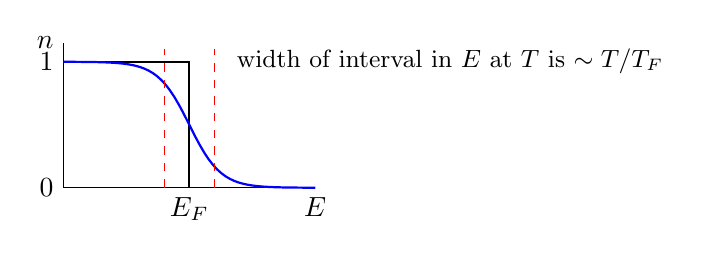
\begin{tikzpicture}[scale=0.8]
  \draw (0,0) -- (4,0) node[below] {$E$}; \draw (0,0) -- (0,2.3) node[left] {$\ev n$};
  \draw[thick] (0,2) -- (2,2) -- (2,0);
  \draw[thick,blue,domain=0:4,samples=60] plot (\x,{2/(exp((\x-2)/0.25)+1)});
  \draw[dashed,red] (1.6,0) -- (1.6,2.2); \draw[dashed,red] (2.4,0) -- (2.4,2.2);
  \node[left] at (0,2) {$1$}; \node[left] at (0,0) {$0$}; \node[below] at (2,0) {$E_F$};
  \node[font=\small,anchor=west] at (2.6,2.0) {width of interval in $E$ at $T$ is $\sim T/T_F$};
\end{tikzpicture}
\diagramcaption{The Fermi--Dirac distribution for $T\ll T_F$; the width of the smeared region $\to 0$ as $T/T_F\to 0$.}
\end{diagram}

So of the total number of electrons, $N_e$, only a very small fraction $N_{e,\text{eff}}\sim\left(T/T_F\right)N_e$ are in states with
$E>E_F$. The rest are in the Fermi sea and are not available to absorb energy. So
\begin{equation}
  U_{\text{K.E.}}\sim N_{\text{eff}}\cdot\left(\frac{3}{2}\kB T\right)\sim N_e\left(\frac{T}{T_F}\right)\left(\frac{3}{2}\kB T\right),
\end{equation}
with $(3/2)\kB T$ the kinetic energy for a free e in the Fermi gas, so the contribution of these conduction electrons to the specific
heat is
\begin{equation}
  C_{v,e} = \frac{\dd U_{\text{K.E.}}}{\dd T}\sim\frac{3N\kB T}{T_F}\ll\frac{3}{2}N_e\kB .
\end{equation}
Combining this contribution to $C_v$ from e's with the contribution from quantized lattice vibrations (phonons), one has the result, at
$T\ll T_D\ll T_F$:
\begin{equation}
  C_v\sim a_1T + a_3T^3 .
\end{equation}
This provides an excellent fit to data in this low-temperature range.
